\section{Benchmark Implementation}
\label{cha:implementation}

This section outlines the implementation details of the benchmark, focusing on three main aspects: (1) service instance configurations, (2) workload generation, and (3) data analysis.

For EC2-Pairs, the benchmarking process is straightforward, with the EC2 instance generating workload on datastores using k6 and storing the collected data locally. For Lambda-Pairs, each Lambda invocation corresponds to a single read operation on the datastore. To invoke the Lambda function programmatically and collect results, an additional EC2 instance, termed "Lambda-Helper", is provisioned with k6 and the necessary test scripts, as shown in \cref{fig:impl_overview}.

All benchmarking runs are executed in the \textit{eu-central-1} AWS region. All components of a run are provisioned and de-provisioned using Infrastructure-as-Code combined with shell scripting. This approach ensures a fresh environment for every run and minimizes the potential for human error. Upon successful completion of a run, the collected data is exported to a dedicated S3 bucket. Additionally, to keep network conditions and resource allocation identical, no benchmarking runs are executed simultaneously.

\begin{figure}[h]
	\centering
	\begin{subfigure}{0.40\linewidth}
		\centering
		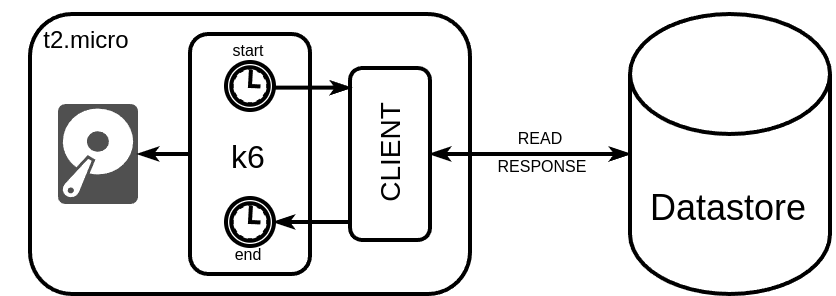
\includegraphics[width=\linewidth]{./fig/ec2-pairs.png}
		\caption{EC2 based Pairs}
		\label{fig:impl_ec2_pairs}
	\end{subfigure}
	\hspace{1cm}
	\begin{subfigure}{0.46\linewidth}
		\centering
		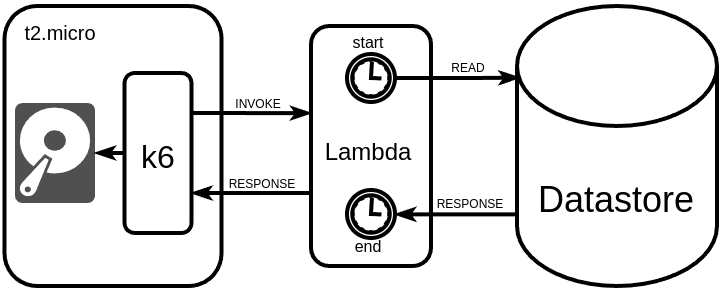
\includegraphics[width=\linewidth]{./fig/lambda-pairs.png}
		\caption{Lambda based Pairs}
		\label{fig:impl_lambda_pairs}
	\end{subfigure}
	\caption{Implementation Overview of EC2 and Lambda with Datastores}
	\label{fig:impl_overview}
\end{figure}

\subsection{Resource Configuration}
\label{sec:config}

\textbf{RDS}:
A MySQL 8.0 instance on a t3.micro VM with 1GiB RAM, 2 vCPUs, and 5GB storage. The instance is located in the \textit{eu-central-1a} AZ, with multi-AZ failover disabled to maintain a single-zone configuration. It hosts a single database containing a table with 1000 rows and four columns.


\textbf{DynamoDB}:
A DynamoDB table in \textit{provisioned capacity} mode with read capacity of 25 RCUs, write capacity of 5 WCUs, and containing 10 items.

\textbf{S3}:
A single S3 bucket with a 20-byte text file.

\textbf{EC2}:
An EC2 instance of t2.micro type with 1GiB RAM, and 1vCPU, located in the \textit{eu-central-1a} AZ. It is operated by Ubuntu Server 24.04 (HVM-based) and is equipped with the k6 and corresponding test scripts.

\textbf{Lambda}:
A non-VPC Node.js 20 function with 1.65GiB RAM, 1vCPU, and reserved concurrency set to 990. The configuration of Lambda-Helper is identical to that of EC2.

\subsection{Workload Generation}
\label{sec:loads}

With the following workload configuration, we specifically address relevance, affordability, and repeatability. However, for relevance, there is no standard rate or load pattern at which, for instance, a backend server reads from a datastore, and depends highly on the application's use case and demand. Instead, we focus on extending the run duration to a point where it can be repeated twice while remaining within the AWS Free Tier. Time limitations are also considered.

\textbf{Constant Workload}:
\begin{itemize}
	\item \textbf{RDS and DynamoDB}: 2 RPS for 14 hours.
	\item \textbf{S3}: 0.2 RPS (1 read every 5 seconds) for 3 hours.
\end{itemize}

\textbf{Burst Workload}:
\begin{itemize}
	\item \textbf{RDS and DynamoDB}: The run starts with a baseline of 2 RPS for the first 2 hours, followed by 30 load spikes. Each spike lasts 3 minutes, with RPS increasing linearly from 2 to 20 in 90 seconds and then decreasing back to the baseline of 2 in 90 seconds. Between spikes, the load remains at 2 RPS for 3 minutes. The run concludes with an additional 2 hours at the 2 RPS, resulting in a total test duration of approximately 7 hours.
	%
	\item \textbf{S3}: The run starts with a baseline of 0.2 RPS for the first 20 minutes, followed by 6 load spikes. Each spike lasts 30 seconds, with RPS increasing linearly from 0.2 to 16 in 15 seconds and then decreasing back to the baseline of 0.2 in 15 seconds. Between spikes, the load remains at 0.2 RPS for 6 minutes. The run concludes with an additional 15 minutes at the 0.2 RPS, resulting in a total test duration of approximately 70 minutes.
\end{itemize}

As noted, the monthly limits for S3 are relatively low, specifically 20000 GET requests per month, which resulted in shorter runs with S3.

\subsection{Data Analysis}
\label{sec:analysis}

As discussed, for each targeted datastore service, we compare latency performance across EC2 and Lambda. Mean values alone cannot fully capture the behavior of access latency throughout the experiment, hence we use bar plots for aggregated metrics and time-series graphs to provide a comprehensive view of the data.

In our context, outliers in latency values may indicate potential network issues between services and can distort analysis, particularly when calculating averages \cite{book_bermbach_cloud_service_benchmarking}. To address this, we identify and remove outliers using the 3-sigma rule, which defines data points beyond three standard deviations from the mean as outliers \cite{book_han_data_mining}. However, the number and extent of these outliers provide valuable insights into a service pair's performance and reliability. Therefore, we also analyze and report outliers to understand their implications and highlight variations between pairs.
